\section{The Standard Model}
\label{sec:sm}
The behaviour of fundamental particles and forces are described by the \sm of
particle physics.
The current formulation of the \sm physics was concocted in the 1970s, when the Higgs
mechanism was incorporated into Glashow's electroweak theory by Salam and Weinberg.
The theory prescribes a treatment
as to how fundamental particles interact via three of the four
fundamental forces, namely: the strong, weak and electromagnetic forces.

Mathematically, the \sm is a locally gauge invariant quantum field theory.
It inhabits a space-time with a global Poincar\'e symmetry that obeys a local
$SU_C(3)\otimes SU_L(2)\otimes U_Y(1)$ symmetry\footnote{
The convention of natural units is used throughout.
Other conventions are that the indices $\mu$ and $\nu$ are used for four vectors, and generators
for the $SU_L(2)$ and $SU_C(2)$ are denoted by $\{i,j,k\}$ and $\{a,b,c\}$, respectively.}.
Each generator in this group corresponds to a spin-1 gauge-boson; so the strong force ($SU_C(3)$ group)
The group $SU_C(3)$ is obeyed by the strong force in the theory of Quantum Chromodynamics (QCD),
while the electroweak sector obeys the $SU_L(2)\otimes U_Y(1)$ gauge group.
Generators for each group correspond to the vector bosons which mediate
interactions --- the eight gluons of the strong force, and the $3+1$ electroweak gauge bosons ($Z$,
$W^\pm$ and the photon).

Spin-$\tfrac12$ particles in the \sm are known as fermions,
which are described by spinor fields, $\psi$, and obey the Dirac equation:
\begin{equation}
  \big(i\gamma^\mu\partial_\mu - m\big)\psi = 0.
  \label{th:eq:dirac}
\end{equation}
The fermions of the \sm can be broadly categorized into \emph{quarks} which couple to the strong
force, and \emph{leptons} which do not.
There are six quarks: up, down, charm, strange, top, and bottom (\uquark, \dquark, \cquark,
\squark, \tquark and \bquark); and six leptons: the electron ($e$), muon ($\mu$), tau ($\tau$), and
their corresponding neutrinos ($\nu_e$, $\nu_\mu$, $\nu_\tau$).
All fermions are organized into pairs forming three generations.
%The fermions of the \sm constitute six leptons (electron, electron neutrino, muon, muon neutrino,
%tau and tau neutrino) and six quarks ($u$p, $d$own, $c$harm, $s$trange, $t$op and $b$ottom), which
%are organized into pairs forming three generations.
For each fermion there is a corresponding antiparticle with the same mass and opposite charge ---
charge being the conserved quantity resulting from the global gauge symmetry (by Noether's
theorem).
There is also a single scalar field in the \sm: the Higgs boson.
%The only additional particle is the scalar Higgs boson.

The \sm Lagrangian can be expressed as a sum of components:
\begin{equation}
  \Lag{SM} = \Lag{QCD} + \Lag{V} + \Lag{\ell} + \Lag{\it q} + \Lag{Higgs} + \Lag{Yuk}.
  \label{eq:th:lag}
\end{equation}
The first term describes interactions of the strong force between colour carrying particles in the
theory of QCD.
The next two terms, \Lag{V} and \Lag{\ell}, encapsulate the weak vector boson self-interactions
and the electroweak behavior of leptons, respectively.
Finally, the remaining terms describe the electroweak behavior of quarks (\Lag{\it q}), the Higgs
interaction (\Lag{Higgs}) and
Yukawa couplings (\Lag{Yuk}).
These latter terms are of fundamental importance as to how flavour, and Charge-Parity (\CP)
violation
arise in the \sm, and will be be discussed in detail.

There are three fundamental discrete symmetryes in the \sm, Charge (C), Parity (P) and Time (T).
Violation of \CP and flavour in the \sm emerges as a direct consequence of the Higgs mechanism
breaking the local electroweak symmetry.
The Higgs doublet, $\Phi$, is a doublet defined to be
\begin{equation}
  \Phi = \frac{1}{\sqrt{2}}
  \begin{pmatrix}
    \phi_1 + i\phi_2 \\
    \phi_3 + i\phi_4 \\
  \end{pmatrix},
  \label{eq:th:phi}
\end{equation}
where each $\phi_i$ is a real field.
The Lagrangian of the Higgs field is:
\begin{align}
  \Lag{Higgs}
  &= \big(D_\mu\Phi\big)^\dagger\left(D^\mu\Phi\right) - V\big(\Phi\big) \nonumber\\
  &= \big(D_\mu\Phi\big)^\dagger\big(D^\mu\Phi\big) - \mu^2\big(\Phi^\dagger\Phi\big) +
  \lambda\big(\Phi^\dagger\Phi\big)^{2},
  \label{eq:th:laghiggs1}
\end{align}
where $\mu$ and $\lambda$ are constants, and $D_\mu$ is the covariant derivative.
Taking $\mu^2<0$ and $\lambda>0$,
as shown in \Fig{fig:th:higgspot},
shifts the minimum of the potential $V(\Phi)$ away from zero by a
distance
\begin{equation}
  v = \sqrt{\frac{\mu^2}{\lambda}}.
\end{equation}
At this point the Higgs field gets a vacuum expectation value (VEV)
of $\langle\phi\rangle = 2^{-\tfrac{1}{2}}v$.
%$\braket{\phi} = \tfrac{1}{\sqrt{2}}v$.
The direction of the VEV from the origin is arbitrary, but the choice of
\begin{align}
  \bra{0}\phi_1\ket{0} =
  \bra{0}\phi_2\ket{0} =
  \bra{0}\phi_4\ket{0} &= 0 \nonumber\\
  \bra{0}\phi_3\ket{0} &= v,
\end{align}
is convenient, and changes the Higgs doublet in \Eq{eq:th:phi} to
\begin{equation}
  \Phi = \frac{1}{\sqrt{2}}
  \begin{pmatrix}
    \eta_1 + i\eta_2 \\
    v + i\eta_4 \\
  \end{pmatrix}.
  \label{eq:th:eta}
\end{equation}
Here, $\eta_1$, $\eta_2$ and $\eta_4$, are Goldstone bosons which, by choosing an appropriate
gauge, become the longitudinal components of the weak vector bosons, and $\Phi$ simplifies to
\begin{equation}
  \Phi = \frac{1}{\sqrt{2}}
  \begin{pmatrix} 0 \\ v+H
  \end{pmatrix}.
  \label{eq:th:phi2}
\end{equation}
The physics Higgs boson is denoted by $H$.
Inserting Eq.~\ref{eq:th:phi2} into Eq.~\ref{eq:th:laghiggs1} gives:
%\begin{multline}
  %\Lag{Higgs} =
  %\frac12\left(\partial_\mu H\right)\left(\partial^\mu H\right)
  %+\frac14g^2\left(v^2 + 2vH + H^2\right)W_\mu^+W^{-\mu}  \\
  %+\frac18\left(g^2 + g^{\prime2}\right)\left(v^2 + 2vH + H^2\right)Z_\mu Z^\mu
  %+ \mu^2H^2 + \frac14\lambda\left(H^4+4vH^3\right) + \cdots,
  %\label{eq:th:laghiggs2}
%\end{multline}
\begin{equation}
  \Lag{Higgs} =
  \frac{1}{2}\big(\partial_\mu H\big)\big(\partial^\mu H\big)
  %+\mu^2H^2
  +\frac{m_H^2}{2}H^2
  +\left(m_W^2W_\mu^+W^{-\mu} + \frac{m_Z^2}{2}Z_\mu Z^\mu\right)
  %\cdot
  \left(1 + \frac{H}{v}\right)^{\!2}
  \label{eq:th:laghiggs2}
\end{equation}
%where $g$ and $g^\prime$ are coupling constants and other terms are three- and four-point
%interactions of the Higgs with itself and weak gauge bosons.
Thus: there is spontaneous symmetry breaking (SSB) of the local $U_Y(1)$ gauge group; weak gauge
bosons become massive, and photons remain massless; as is consistent with observations.

\begin{figure}
  \begin{center}
    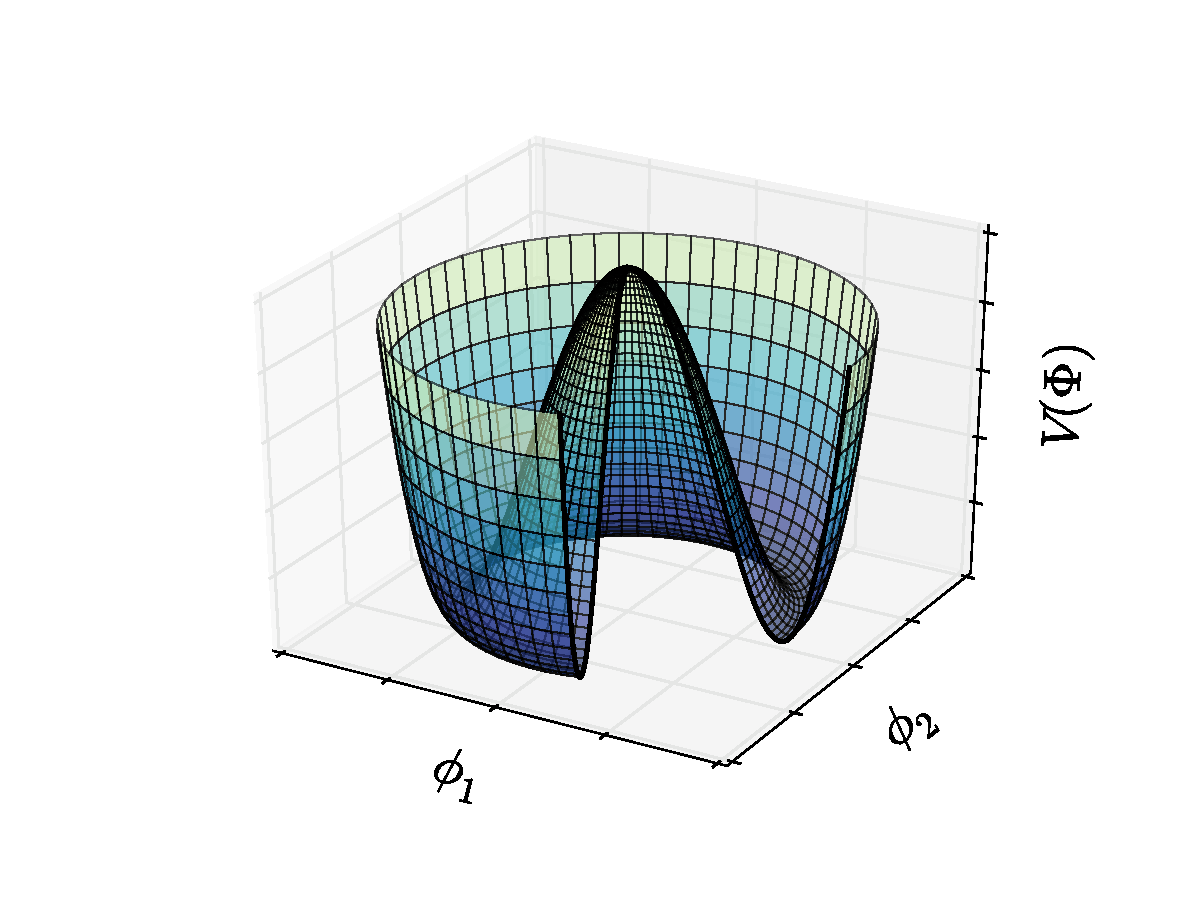
\includegraphics[width=0.6\textwidth]{higgs_potential}
    \caption{\small
      The shape of the Higgs potential, $V(\Phi)$, for the simple case of $\Phi=\phi_1+i\phi_2$ and
      $\mu^2<0$ and $\lambda>0$.
      Spontaneous symmetry breaking occurs when the vacuum settles in a minma, this choice of
      direction breaks the symmetry of the gauge.
      A section of the potential is not shown, in order to appreciate the shape of the potential.
    }
    \label{fig:th:higgspot}
  \end{center}
\end{figure}

%It is not possible to directly insert mass terms for fermions, because the required terms
%($m(\bar\psi_L\psi_R+\bar\psi_R\psi_L$) are not allowed \bam{ELABORATE}.
All fermions (excepting neutrinos) also acquire mass after the SSB.
The Dirac mass term for a chiral field would have the form:
\begin{equation}
  \Lag{mass} = -m_\psi\big(\xbar\psi_R\psi_L + \xbar\psi_L\psi_R\big),
\end{equation}
but the left- and right-handed fields
transform differently under local gauge transformations
--- because $\psi_L$ and $\psi_R$ have different $U(1)$ charges ---
and so cannot be added to \Lag{SM}.
Instead, masses are generated through the Yukawa couplings (\Lag{Yuk} in \Eq{eq:th:lag}), which
describe interactions between all fermionic fields and the Higgs doublet.
This can be written
\begin{equation}
  %\Lag{Yuk} = \sum_{\substack{\ell=\\e,\mu,\tau}}\big(\Lag{Yuk}^\ell\big) + \Lag{Yuk}^q,
  \Lag{Yuk} = \sum_{\ell}\big(\Lag{Yuk}^\ell\big) + \Lag{Yuk}^q,
  \label{eq:th:yukking}
\end{equation}
where terms encapsulate lepton ($\ell\in\{e,\mu,\tau\}$) and quark interactions, respectively.
%where $\ell$ and $q$ denote the lepton and quark interactions, respectively.
Each lepton term describes the interacion between the Higgs boson and and the chiral fields
$\ell_R$ and
\begin{align}
  \chi_L = \begin{pmatrix}\nu_L \\ \ell_L \end{pmatrix},
\end{align}
via
\begin{equation}
  \Lag{Yuk}^\ell
  = - g_\ell\big(\xbar\chi_L\Phi \ell_R + \xbar \ell_R\Phi^\dagger\chi_L\big),
\end{equation}
where $g_\ell$ is a coupling constant.
After SSB the Lagrangian becomes
\begin{align}
  \Lag{Yuk}^\ell
  = - m_\ell \big(\xbar\ell_L\ell_R + \xbar\ell_R\ell_L\big)%\cdot
  \left(1 + \frac{H}{v}\right)
\end{align}
where
\begin{equation}
  m_\ell = \frac{v}{\sqrt{2}}g_\ell.
  \label{eq:leptonmass}
\end{equation}
is the lepton mass and is dependent on the fundamental \sm parameters $g_\ell$ and $v$

Yukawa interactions for quarks involve the right-handed chiral operators of the up- and down-type
quarks, $q_R^i$ for $q\in{u,d}$, and the left-handed doublet
\begin{equation}
  Q_L^i = \begin{pmatrix}u^i_L\\d^i_L\end{pmatrix}.
\end{equation}
Before SSB, the Yukawa Lagrangian is
\begin{equation}
  \Lag{Yuk}^q = - y_{ij}^u\Xbar{Q}_L^i\Phi u_R^j
  - y_{ij}^d\Xbar{Q}_L^i\widetilde\Phi d_R^j + \mathrm{h.c.}
  \label{eq:th:lagyukq}
\end{equation}
where $\widetilde\Phi_i = \varepsilon_{ij}\Phi_k$ and there is an implict sum over the generations
$i$ and $j$.
The coupling constants, $y^{q}$, are $3\times3$ matrices characterizing Yukawa coupling strengths
between generations.
After SSB, and the Higgs acquires a VEV, \Lag{Yuk} becomes:
\begin{equation}
  \Lag{Yuk}^q =
  - \frac{v}{\sqrt{2}}
  \left(
  y_{ij}^\uquark\uquarkbar_L^i\uquark_{R,j}
  + y_{ij}^\dquark\dquarkbar_L^i\dquark_{R,j},
  + \mathrm{h.c.}
  \right)
  %\cdot
  \left(1 + \frac{H}{v}\right).
  \label{eq:th:lagyuk2}
\end{equation}
Similar to lepton masses, in \Eq{eq:leptonmass}, quark mass are defined as
\begin{align}
  m_{ij}^u = -\frac{v}{\sqrt{2}}y_{ij}^u &&
  m_{ij}^d = -\frac{v}{\sqrt{2}}y_{ij}^d.
\end{align}
However, it is more convenient to change to a basis in which the matrix $m^q$
is diagonal, using the rotation matrices $V_L$ and $V_R$
\begin{align}
  {m_{il}^{u}}^\prime =  \big(V_L^{u\dagger}\big)_{ij} m_{jk}^u\big(V_R^u\big)_{kl} &&
  {m_{il}^{d}}^\prime =  \big(V_L^{d\dagger}\big)_{ij} m_{jk}^d\big(V_R^d\big)_{kl}.
\end{align}
The mass basis is distinguished from the flavour basis by the addition of a prime.
This transformation is exactly equivalent to transforming the up- and
down-type chiral quark fields according to:
\begin{align}
  q_L^\prime = \big(V_L^q\big)q_{L}^{} &&
  q_R^\prime = \big(V_R^q\big)q_{R}^{}.
\end{align}
Applying these transformations to all parts of \Lag{SM} leaves the majority of it unchanged, since
$V_{L}^{q\dagger} V_{L}^{q} = V_{R}^{q\dagger} V_{R}^{q} = \mathds{1}$ by definition.
%$m_{ij}^\mathrm{diag} = V_{Lik}m_{kl}(V_R^\dagger)_{lj}$.
%This is exactly equivalent to transforming the chiral quark fields for up- and down-type quarks
%accordingly:
%\begin{align}
  %q_L^\alpha = \left(V_L^q\right)_{\alpha i}q_L &&
  %q_R^\alpha = \left(V_R^q\right)_{\alpha i}q_R,
%\end{align}
%where the index of the original basis is identified with $i$ and the mass basis uses $\alpha$.
%The rotations of the basis of the chiral quark fields leave much of \Lag{SM} unchanged since
%$V_{qL}^\dagger V_{qL} = V_{qR}^\dagger V_{qR} = \mathbb{1}$.
However, this is not the case of \Lag{\it q}.

The Lagrangian $\Lag{\it q}=\Lag{\it q}^\mathrm{NC}+\Lag{\it q}^\mathrm{CC}$, where the
superscripts denote neutral current (NC) and charged current (CC) components.
The neutral current part characterizes interactions between quarks and the neutral electroweak
vector boson.
In the charged current (CC) part of \Lag{\it q}; which transforms as:
\begin{align}
  \Lag{\it q}^\mathrm{CC}
  &= i\frac{g}{2}\gamma^\mu
  \bigg[\uquarkbar_Ld_LW^+_\mu + \dquarkbar_Lu_LW^-_\mu
  \bigg]  \nonumber\\
  &= i\frac{g}{2}\gamma^\mu
  \bigg[
    \uquarkbar_L^\prime\left(V_{uL}^{\phantom{\dagger}}V_{dL}^\dagger\right)d_L^{\,\prime} W^+_\mu +
    \dquarkbar_L^{\,\prime}\left(V_{dL}^{\phantom{\dagger}}V_{uL}^\dagger\right)u_L^\prime W^-_\mu
  \bigg]  \nonumber\\
  &= i\frac{g}{2}\gamma^\mu
  \bigg[
    \VCKM\uquarkbar_L^\prime d_L^{\,\prime} W^+_\mu +
    \VCKMconj\dquarkbar_L^{\,\prime} u_L^\prime W^-_\mu
  \bigg].
\end{align}
The matrix $\VCKM=V^{\phantom{\dagger}}_{uL}V_{dL}^\dagger$ is known as the \ckm
matrix and parameterizes the couplings between up- and down-type quarks in charged weak currents.



